\documentclass[12pt]{report}
\usepackage[utf8]{inputenc}
\usepackage{amsmath}
\usepackage{amsfonts}
\usepackage{amssymb}
\usepackage[pdftex]{graphicx}
\usepackage{polski}

\usepackage{placeins}
\usepackage{epstopdf}
\usepackage{mathtools}
\usepackage{amsthm}
\usepackage{float}
\usepackage{tabularx}
\usepackage{titlesec}

\titleformat{\chapter}
{\Large\bfseries} % format
{}                % label
{0pt}             % sep
{\huge}           % before-code


\usepackage[left=2.50cm, right=2.50cm, top=2.50cm, bottom=2.50cm]{geometry}

\newcolumntype{C}[1]{>{\hsize=#1\hsize\centering\arraybackslash}X}
\newcolumntype{M}[1]{>{\centering\arraybackslash}m{#1}}

%opening
\title{\textbf{SCADA 2}}
\author{Maciej Cebula \\Piotr Merynda \\Maciej Podsiadło}
\date{}
\begin{document}
	
%	\fancypagestyle{plain}
%	{
%		% Usuń nagłówek i stopkę
%		\fancyhf{}
%		% Usuń linie.
%		\renewcommand{\headrulewidth}{0pt}
%		\renewcommand{\footrulewidth}{0pt}
%	}

	
	\setcounter{tocdepth}{2}
	
	\maketitle
	\tableofcontents
	\clearpage
		
		\renewcommand{\tablename}{Tabela}
		\renewcommand{\figurename}{Rys.}
		
	\chapter{Wstęp}

\section{Opis projektu}



\section{Założenia}


	\chapter{Serwer HTTP}
\section{Opis działania}
W celu umożliwienia komunikacji aplikacji wizualizującej z bazą danych napisano w języku \textit{JAVA} serwer HTTP. Dane pomiędzy serwerem i aplikacją wymieniane są za pomocą protokołu HTTP, wykorzystując w tym celu zapytania typu \textit{GET} i \textit{POST}. Wszystkie żądania są utożsamione z odpowiednim adresem url i odpowiednio przetwarzane po stronie serwerowej. Aby zapewnić jak największą responsywność aplikacji oraz synchroniczne odświeżanie danych każdy request po stronie serwera przetwarzany jest w osobnym wątku. \\
Do napisania serwera wykorzystano następujące biblioteki \textit{JAV-wy}:
\begin{enumerate}
	\item \textbf{RXJava} - biblioteka zapewniająca mechanizmy asynchronicznego przetwarzania danych \cite{rxjava},
	\item \textbf{JDBI} - biblioteka zapewniająca połączenie z bazą danych \cite{jdbi},
	\item \textbf{AKKA-HTTP} - framework do implementacji serwera HTTP \cite{akka doc},
	 \item \textbf{Javax mail} - biblioteka do wysyłania emaili.
\end{enumerate}

\section{Uruchomienie serwera}
W momencie pisania sprawozdania w repozytorium \textit{} nie udostępniono jeszcze skompilowanej wersji flików \'zródłowych. Dlatego też w celu uruchomienia aplikacji na komputerze wymagane jest: 
\begin{enumerate}
	\item zainstalowanie Jav-y w wersji 8
	\item zainstalowanie dowolnego środowiska programistycznego \textit{Intellij, Eclipse itp.}
	\item skompilowanie i uruchomienie całego projektu dostępnego pod adresem \\ \textit{https://github.com/maciekc/SCADA2}
\end{enumerate}
	\chapter{Baza danych}

\section{Wstęp}
Aby móc wizualizować przebieg pracy systemu wszystkie najważniejsze dane z punktu widzenia automatyki są logowane w bazie danych. Do tego celu wykorzystano bazę danych typu \textit{MYSQL} i środowisko \textit{MYSQL Workbench}, zainstalowane na jednym z komputerów, którym stworzono całą strukturę przedstawioną na rysunku \ref{fig:db}. Dostęp poszczególnych węzłów systemu do bazy danych zapewniony jest poprzez połączenie wszystkich komputerów w lokalną sieci. 
 

\section{Struktura bazy}

Zaprezentowana na rysunku baza danych na strukturę relacyjną aby zapewnić możliwość ewentualnej rozbudowy sytemu o inne składowe. Z racji na to, że baza służy głównie do logowania pracy systemu podzielono ją na następujące części:
\begin{enumerate}
	\item główną tabele \textbf{history}, w której logowane są wszystkie zdarzenia w kolejności chronologicznej,
	\item tabelę  \textbf{Andon}, w której zapisywane są wszystkie sytuacje alarmowe,
	\item tabelę \textbf{Work}, do której logowany jest stan normalnej pracy systemu,
	\item tabelę \textbf{change\_parameter}, w której zapisywane są wszelkie zmiany wartości parametrów systemu,
	\item tabelę \textbf{controller}, która służy do logowania pracy regulatorów.
\end{enumerate}
%
Dodatkowo:
\begin{enumerate}
	\item w tabeli \textbf{state\_space} zdefiniowano wszystkie zmienne stanu występujące w systemie,
	\item tabele \textbf{variable\_state} definiuje wszystkie możliwe stany danej zmiennej np. Work, Andon, Change parameter itd.
	\item tabela \textbf{limits} definiuje poszczególne limity i przypisuje je do odpowiednich zmiennych stanu z tabeli \textbf{state\_space},
	\item w tabeli \textbf{system\_parameter} zdefiniowane są pozostałe parametry systemu takie jak: nastawy poszczególnych regulatorów, wartości zadane itp.
\end{enumerate}

\newpage
\begin{figure}[H]
	\centering
	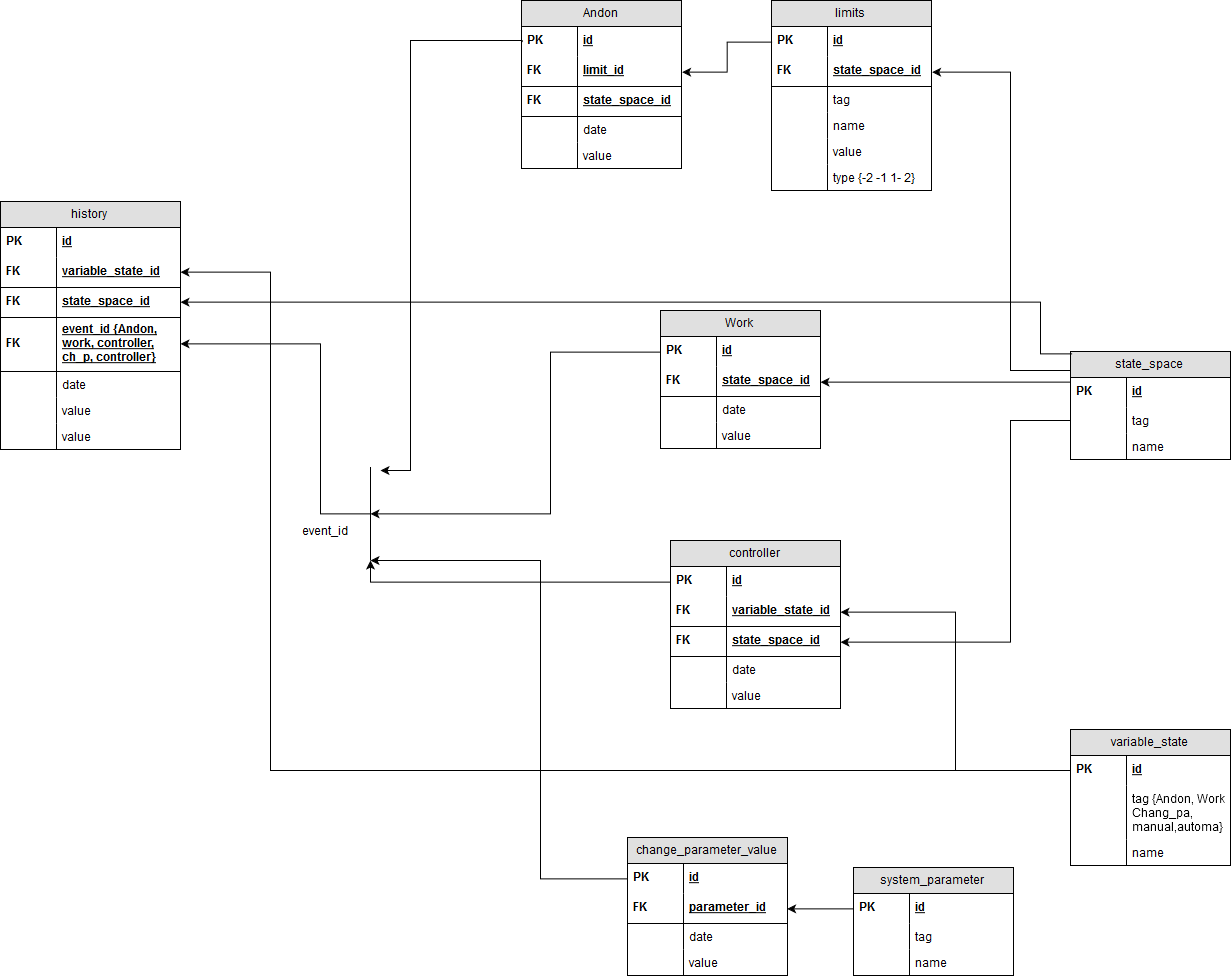
\includegraphics[scale = 0.4]{fig/DB_SCHEMA.png}
	\caption{Struktura bazy danych.}
	\label{fig:db}
\end{figure}

\section{Opis dostępu do bazy}

Dane dotyczące parametrów systemu w poszczególnych chwilach czasu są logowane przez serwer OPC i następnie prezentowane w aplikacji.  
	\section{Serwer OPC}
\subsection{Wprowadzenie}
Systemy typu PLC – SCADA są powszechnie wdrażane poczynając od przemysłu chemicznego, a kończąc na automatyce budynków. Stanowią pewną normę w nowoczesnych zakładach oraz fabrykach. W związku z bogatą ofertą producentów aparatury automatyzacji powstał problem komunikacji pomiędzy różnymi komponentami. Firmy promowały swoje rodzime protokoły przemysłowe, co wymuszało na końcowych użytkownikach stosowanie sprzętu pochodzącego od tego samego producenta w obrębie całego obiektu. Przełomem okazało się wprowadzenie otwartego rozwiązania – standardu OPC. OPC jest standardem umożliwiającym komunikację pomiędzy sterownikami (najczęściej PLC) a oprogramowaniem SCADA. Bazuje na modelu klient-serwer, przy czym strona serwera zaimplementowana jest w oprogramowaniu dostarczanym przez producentów sterowników, natomiast klientem - aplikacja wykorzystująca udostępniane dane. 
\subsection{MatrikonOPC}
Dla celów zintegrowania omawianego systemu zastosowano testowy serwer udostępniony przez firmę Matrikon służący do celów niekomercyjnych. Dostawca oferuje serwer OPC (OPC Simulation Server), jak również oprogramowanie do zarządzania odczytywanymi danymi (OPC Explorer). 
%TODO konfiguracja serwera
\subsection{Logowanie OPC - MySQL}
Kolejny element stworzonego wielopoziomowego systemu sterowania stanowi aplikacja logująca aktualne dane pochodzące z serwera OPC do procesowej bazy danych. Aplikacja napisana została w języku C\#. Do komunikacji z serwerem użyto open sourcową bibliotekę TitaniumAS.Opc (https://github.com/titanium-as/TitaniumAS.Opc.Client). Serwer lokalizowany jest jedynie po nazwie, co, zgodnie z ideą OPC, znacząco przyspiesza proces integracji. Aplikacja odczytuje bieżące pomiary z serwera OPC z zadaną przez użytkownika częstotliwością, a następnie loguje je w bazie danych MySQL. Podstawową częstotliwością odpytywania jest 1 sekunda, tak jak to ma miejsce w większości systemów typu SCADA. Poszczególne pomiary identyfikowane są po tagach jakie zostały im nadane w momencie inicjalizacji w serwerze OPC. Zapis do bazy danych odbywa się według konwencji narzuconej w momencie jej zaprojektowania. Aplikacja zapewnia mechanizmy przechwytywania zgłaszanych błędów, w szczególności błędów połączenia z serwerem oraz MySQL. Użytkownik informowany jest o napotkanym błędzie. Program dokonuje niezbędnej konwersji sposobu zapisu liczb zmiennoprzecinkowych, zamienia separator ‘,’ na ‘.’ bez czego zapis do bazy danych nie byłby możliwy.
 
Warto nadmienić, że użytkownik operujący na systemie Windows nie musi instalować, żadnego dodatkowego oprogramowania w celu uruchomienia omawianej aplikacji logującej.

	\begin{thebibliography}{}
	
	%przykład 
	
%	\bibitem{pauluk 1}Pauluk, M.: 
%	\emph{Model matematyczny trójwymiarowej suwnicy.} W: \textbf{Automatyka} 2002 tom 6 s. 69-102, ISSN: 1429-3447
%	

	
\end{thebibliography}
	
\end{document}